% Section 06 - Manipulate Conductivity in Quantum Hall Systems

To identify the characteristics of the transverse conductivity of the quantum Hall systems with external dressing field, first we can derive a expression for a normalized
transverse conductivity as a function of fermi energy $X_F$ and intensity of the dressing field $I$. Here we have the normalized x-directional conductivity using the natural conductivity of least Landau level
\begin{equation} \label{eq_35}
  \begin{aligned}
    \sigma^{xx}/\sigma^{0} = &
    \sum_{n}
    \frac{\qty(n+1)}{0.0037\Lambda_n \Lambda_{n+1}} \\
    & \times
    \qty[
      \frac{1}
      {
        1 + \qty(\frac{X_F - n -1}{0.06\Lambda_n})^2
      }
    ]
    \qty[
      \frac{1}
      {
        1 + \qty(\frac{X_F - n}{0.06\Lambda_{n+1}})^2
      }
    ]
  \end{aligned}
\end{equation}
where $\sigma^0 = (e^2/\pi \hbar A)$. We use this expression to illustrate the changes that can be done to the transverse conductivity in 2DEG using external dressing field. As given in Fig.~\ref{fig_4} and \ref{fig_5} we can manipulate the transverse conductivity $\sigma_{xx}$ using external dressing field's intensity and the Fermi level $X_F$ of the considering system. For a given dressing field intesity, the transverse conductivity vary against the Fermi level of the system by creating sharp peaks at each Landau level energy values. Since electrons are restricted to have only Landau level energies, the conductivity gets very low values when the Fermi level is not align with any of the Landau level energy values. In contrast, on Landau levels conductivity can achieve very high values compared to other areas and as illustrates on Fig.~\ref{fig_4} the peak value of transverse conductivity on each Landau level gets increase with the Landau level number.

\begin{figure}[t]
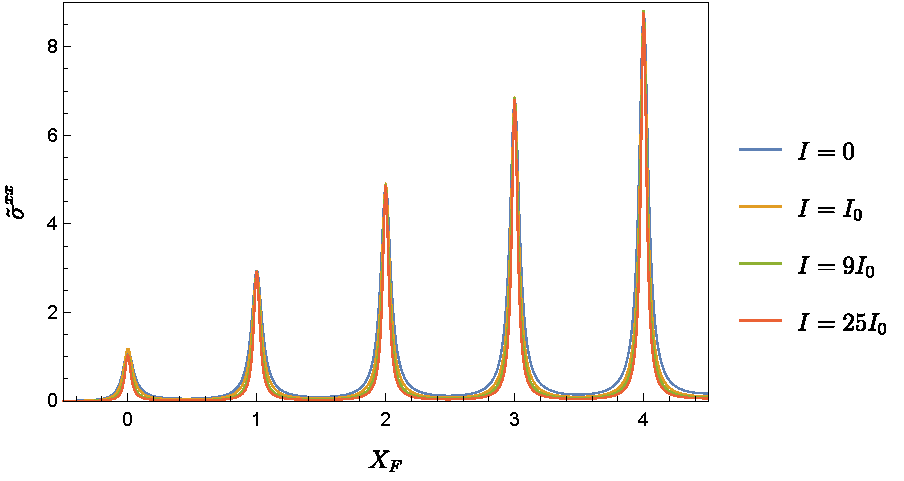
\includegraphics[scale=0.55]{figures/fig_5}
\caption{\label{fig_5} Normalized transverse conductivity $\sigma_{xx}$ against Fermi level $X_F$ with different intensities $I$ of the external dressing field in a GaAs-based quantum well at a magnetic field $B = 1.2~\text{T}$, dressing field with frequency $\omega =2\times10^{12}~\text{rad}\text{s}^{-1}$ and $I_0 =100~\text{W}/\text{cm}^{2}$. In this calculation we have assumed that the natural  broadening of $0$-th Landau level $\Gamma_0$ is $0.24\;\text{me}V$.}
\end{figure}
\begin{figure}[t]
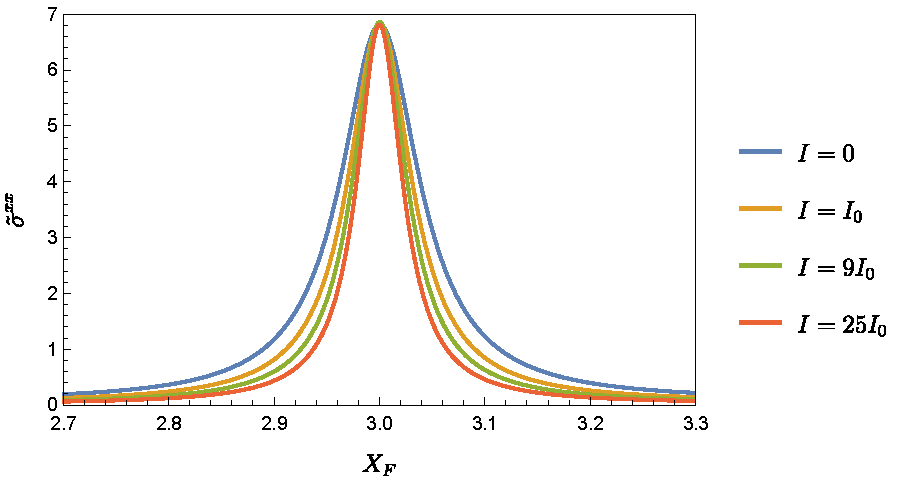
\includegraphics[scale=0.55]{figures/fig_6}
\caption{\label{fig_6} $3$rd Landau level’s normalized transverse conductivity $\sigma_{xx}$ against Fermi level $X_F$ with different intensities $I$ of the external dressing field in a GaAs-based quantum well at a magnetic field $B = 1.2~\text{T}$, dressing field with frequency $\omega =2\times10^{12}~\text{rad}\text{s}^{-1}$ and $I_0 =100~\text{W}/\text{cm}^{2}$. In this calculation we have assumed that the natural  broadening of $0$-th Landau level $\Gamma_0$ is $0.24\;\text{me}V$}.
\end{figure}

Considering the effect of the external dressing field on transverse conductivity of 2DEG, we can identify that high intensities shrink the conductivity regions near Landau levels. However the peak value of the conductivity at each Landau level has the same value as the undressed system. This demostrate that we are able to tune the width of the regions of conductivity in these quantum Hall systems with the help of a dressing field.
These characteristics are align with results demostrated by K. Dini et al.\cite{dini16} and as they remarked since the Fermi level of the system can be change with the applied gate voltage of the material this can be used as a 2D switch for optoelectonic applications. Controlling  the external dressing field we are able to fine-tune the switching mechanism for optimized performance.
Furthermore we can distinguish that the shapes and behavoiur of the conductivity regions illustrated in Fig.~\ref{fig_4} and \ref{fig_5} are generally incompatible with the results reported in Ref.~\cite{dini16}. This is due to the selection of the conventional transverse conductivity theory of 2DEG from Ref.~\cite{ando74_1,ando82}. The semi-elliptical conductivity regions illustrated in Ref.~\cite{dini16,ando74_1,ando82}, have less consistance with the experimentally observed Landau levels representation \cite{endo09}.
In our study on the transport properties of quantum Hall systems, we developed the conductivity expression starting from Floquet-Drude conductivity \cite{wackerl20} and our results are much more align with the result represented by A. Endo et al. \cite{endo09}.
The description of conductivities of quantum Hall systems demostrated in Ref.~\cite{endo09} has excellent agreement between the theory and experiment obtained in a GaAs/AlGaAs 2DES for the low magnetic field range. However they have not consider about the tunability that can be achived with the external strong dressing field. In this analysis we account both magnetic and dressing field effects that can be applied into the transport properties of 2DEG and we have presented a more generalized theory. As a concluding remark, in this study we were able to demonstrate that using Floquet-Drude conductivity method one can derive a more experimental fitting and generalized mathematical model that describes the trasport properties of quantum Hall syatems.
